\chapter{Introduction au domaine}

\section{Modèles}
Le principal modèle développé est celui des créatures.
Ce modèle permet de simuler l'évolution d'une espèce dans un milieu donné.
Il utilisera le réseau de neurones comme ``attribut de classe''\\
Les individus (les créatures) doivent pour survivre, boire de l'eau, éviter le feu et ramener des diamants à la maison.
\\Pour bouger, les créatures ont en entrée la possibilité de détecter si :\\

\begin{itemize}
 \item un diamant est devant soi
 \item de l'eau est devant soi
 \item du feu est devant soi
 \item la maison est devant soi
 \item transporte actuellement un diamant\\
\end{itemize}

La créature à possibilité de :
\begin{itemize}
 \item tourner à gauche
 \item tourner à droite
 \item avancer\\
 
 \end{itemize}
 
 Le choix des actions est déterminé par les poids associés à chaque réseau de neurones d'une créature.\\

Dans un second temps, un modèle basé sur la bourse (ex: CAC40) est envisagé.
Il utilisera aussi le réseau de neurones déjà implémenté.

\section{Réseau de neurones}
Ecrire ici

    %\centering
    %
\includegraphics[width=0.4\textwidth]{./pictures/neurone.png}
   
\begin{figure}[H]
    \centering
    
\includegraphics[width=0.8\textwidth]{./pictures/neurone.png}
    \caption{Exemple de neurone}
    \label{fig:awesome_image}
\end{figure}


\section{Algorithme génétique}
Les algorithmes génétiques sont des algorithmes s'inspirant de l'évolution des especes, leur but est de trouver une solution (qui n'est pas forcement optimale), en un temps raisonnable. Ils vont à partir d'un problème donné, chercher une solution selon le processus suivant: 
- création d'une population initiale
- évaluation de la population
- sélection, reproduction, mutation
- insertion des nouveaux individus dans la population

I – Création de la population initiale

	Au début de notre programme, la population est créée aléatoirement: c'est a dire que les gènes attribués aux individus sont aléatoires. C'est à partir de celle-ci que nous allons réaliser les tests, de plus, cette population ne répondra pas forcement aux critères de sélection, elle devra cependant être cohérente par rapport à son environnement: par exemple, si l'on code un jeu, ces individus devront respecter les règles du jeu, mais ne sont pas obligés de donner une solution au problème.

II – Évaluation de la population

	Notre population initiale étant créée, cette étape consiste maintenant à évaluer les individus dans leur environnement selon plusieurs critères définis et a leur attribuer un score.

III – Sélection, reproduction, mutation

	Cette étape permet la création d'une nouvelle génération: nous allons tout d'abord sélectionner les différents individus qui seront ensuite utilisés pour la création d'une nouvelle génération, puis nous allons croiser leurs gènes, enfin une mutation peut être introduite chez certains individus de la nouvelle génération.
 
	Il existe plusieurs modes de sélection d'individus tel que la selection par rang, la selection par tournoi, etc. (Detailler un peu plus cette partie)
	Le croisement des genes des individus peut se faire aleatoirement, cependant il existe une solution qui est largement plus répendue: les croisements multi-points(a detailler).
	Durant cette étape, on va egalement appliquer à certains individus (un tres faible pourcentage), une mutation génétique: de façon aléatoire, un gene peut être substitué à un autre.

IV – Creation de la nouvelle generation

	Une fois la nouvelle generation créée, on lui applique les mêmes tests d'évaluation et modes de selection que la génération précédentes.

Mettre image du fonctionnement de l'algorithme

Le programmeur peut choisir le nombre de génération a créer: généralement, une solution est trouvée en moins de 10 générations, et au bout de 500 générations, les solutions n'évoluent plus, cependant rien ne garantit que nous obtenions une solution optimale.

Nous pouvons donc en conclure que les algorithmes génétiques offrent une grande liberte de parametrage et d'implementation au programmeur, ce qui en fait un outil utilisé dans plusieurs domaines de recherche.


\begin{figure}[H]
    \centering
    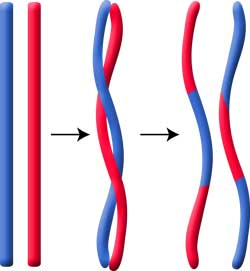
\includegraphics[width=0.2\textwidth]{./pictures/adn.jpg}
    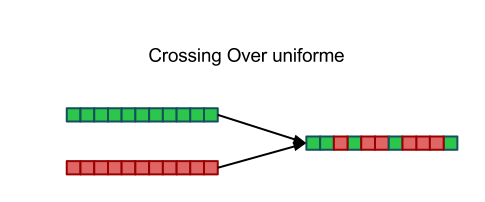
\includegraphics[width=0.8\textwidth]{./pictures/reproduction.png}
    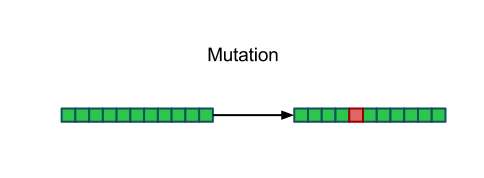
\includegraphics[width=0.8\textwidth]{./pictures/mutation.png}
    
    \caption{Exemple : Algorithme génétique}
    \label{fig:awesome_image}
\end{figure}

\clearpage
